\let\negmedspace\undefined
\let\negthickspace\undefined
\documentclass[journal]{IEEEtran}
\usepackage[a5paper, margin=10mm, onecolumn]{geometry}
%\usepackage{lmodern} % Ensure lmodern is loaded for pdflatex
\usepackage{tfrupee} % Include tfrupee package

\setlength{\headheight}{1cm} % Set the height of the header box
\setlength{\headsep}{0mm}     % Set the distance between the header box and the top of the text

\usepackage{gvv-book}
\usepackage{gvv}
\usepackage{cite}
\usepackage{amsmath,amssymb,amsfonts,amsthm}
\usepackage{algorithmic}
\usepackage{graphicx}
\usepackage{textcomp}
\usepackage{xcolor}
\usepackage{txfonts}
\usepackage{listings}
\usepackage{enumitem}
\usepackage{mathtools}
\usepackage{gensymb}
\usepackage{comment}
\usepackage[breaklinks=true]{hyperref}
\usepackage{tkz-euclide} 
\usepackage{listings}
% \usepackage{gvv}                                        
\def\inputGnumericTable{}                                 
\usepackage[latin1]{inputenc}                                
\usepackage{color}                                            
\usepackage{array}                                            
\usepackage{longtable}                                       
\usepackage{calc}                                             
\usepackage{multirow}                                         
\usepackage{hhline}                                           
\usepackage{ifthen}                                           
\usepackage{lscape}
\begin{document}
\bibliographystyle{IEEEtran}
\title{5.2.5}
\author{EE25BTECH11002 - Achat Parth Kalpesh }
{\let\newpage\relax\maketitle}
\renewcommand{\thefigure}{\theenumi}
\renewcommand{\thetable}{\theenumi}
\setlength{\intextsep}{10pt} % Space between text and floats
\numberwithin{equation}{enumi}
\numberwithin{figure}{enumi}
\renewcommand{\thetable}{\theenumi}
\parindent 0px



\textbf{Question:}\\
Solve the following system of linear equation
\begin{align}
    3x + 2y = 5\\
    2x - 3y = 7
\end{align}

\textbf{Solution:}\\
The above equation can be written as
\begin{align}
    \myvec{3 & 2\\2 & -3}\myvec{x\\y} = \myvec{5\\7}
\end{align}

Performing row operations:
\begin{align}
    \augvec{2}{1}{3 & 2 & 5 \\ 2 & -3 & 7}
    &\xleftrightarrow[]{R_1 \leftarrow \frac{R_1}{3}} 
    \augvec{2}{1}{1 & \frac{2}{3} & \frac{5}{3} \\ 2 & -3 & 7} \\
    \augvec{2}{1}{1 & \frac{2}{3} & \frac{5}{3} \\ 2 & -3 & 7}
    &\xleftrightarrow[]{R_2 \leftarrow R_2 - 2R_1} 
    \augvec{2}{1}{1 & \frac{2}{3} & \frac{5}{3} \\ 0 & -\frac{13}{3} & \frac{11}{3}} \\
    \augvec{2}{1}{1 & \frac{2}{3} & \frac{5}{3} \\ 0 & -\frac{13}{3} & \frac{11}{3}}
    &\xleftrightarrow[]{R_2 \leftarrow -\frac{3}{13}R_2} 
    \augvec{2}{1}{1 & \frac{2}{3} & \frac{5}{3} \\ 0 & 1 & -\frac{11}{13}} \\
    \augvec{2}{1}{1 & \frac{2}{3} & \frac{5}{3} \\ 0 & 1 & -\frac{11}{13}}
    &\xleftrightarrow[]{R_1 \leftarrow R_1 - \frac{2}{3}R_2} 
    \augvec{2}{1}{1 & 0   & \frac{29}{13} \\ 0 & 1   & -\frac{11}{13}}
\end{align}
Thus,
\begin{align}
    \vec{x} = \myvec{\frac{29}{13}  \\  -\frac{11}{13}}
\end{align}


\begin{figure}[h]
    \centering
    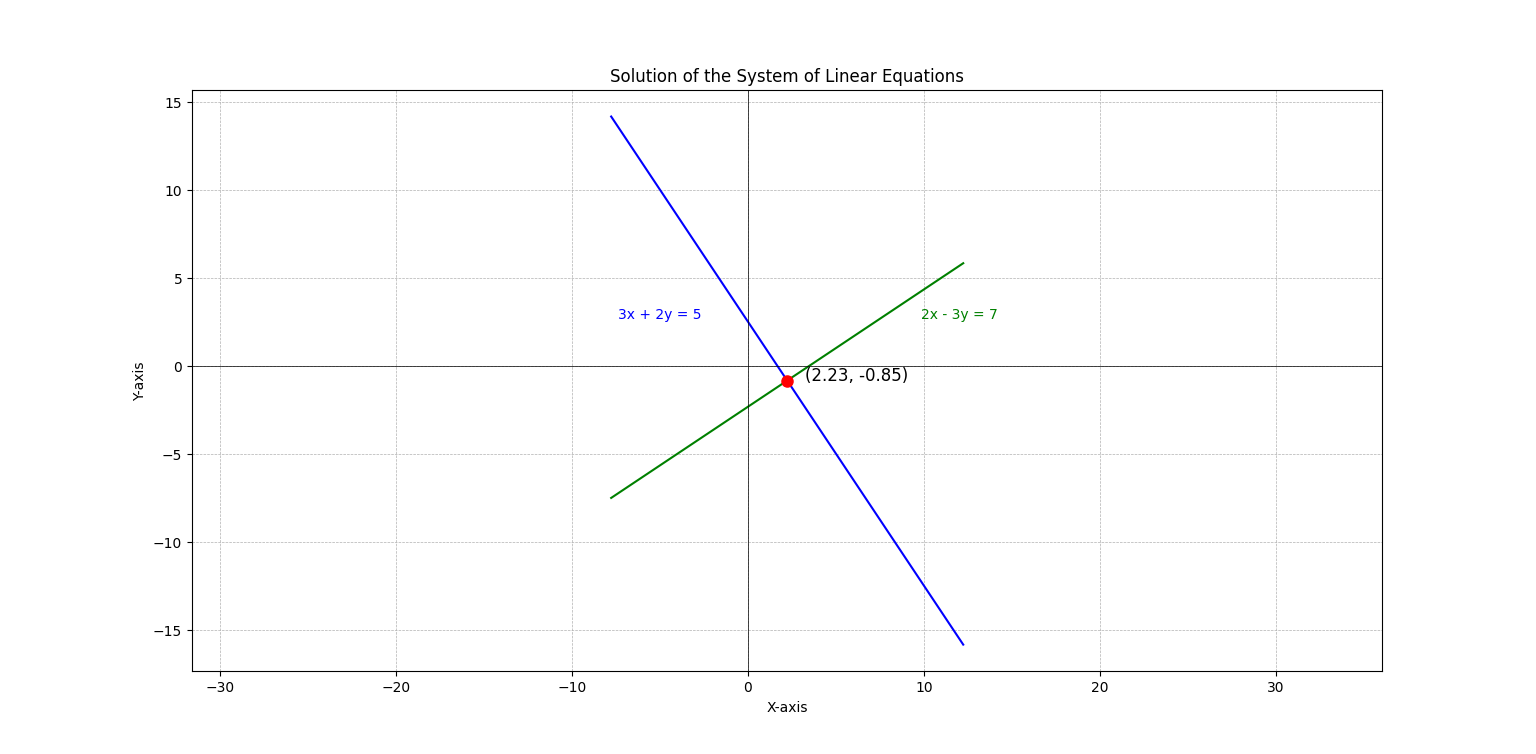
\includegraphics[width=0.7\columnwidth]{figs/figure_py.png}
    \caption{Graph}
    \label{fig:fig}
 \end{figure}
\end{document}